%%%%%%%%%%%%%%%%%%%%%%%%%%%%%%%%%%%%%%%%%%%%%%%%%%%%%%%%%%%%%%%%%%
%%%%%%%% ICML 2014 EXAMPLE LATEX SUBMISSION FILE %%%%%%%%%%%%%%%%%
%%%%%%%%%%%%%%%%%%%%%%%%%%%%%%%%%%%%%%%%%%%%%%%%%%%%%%%%%%%%%%%%%%

% Use the following line _only_ if you're still using LaTeX 2.09.
%\documentstyle[icml2014,epsf,natbib]{article}
% If you rely on Latex2e packages, like most moden people use this:
\documentclass{article}

% use Times
\usepackage{times}
% For figures
\usepackage{graphicx} % more modern
%\usepackage{epsfig} % less modern
\usepackage{subfigure}

% For citations
\usepackage{natbib}

% For algorithms
\usepackage{algorithm}
\usepackage{algorithmic}

% As of 2011, we use the hyperref package to produce hyperlinks in the
% resulting PDF.  If this breaks your system, please commend out the
% following usepackage line and replace \usepackage{icml2014} with
% \usepackage[nohyperref]{icml2014} above.
\usepackage{hyperref}

% Packages hyperref and algorithmic misbehave sometimes.  We can fix
% this with the following command.
\newcommand{\theHalgorithm}{\arabic{algorithm}}

% Employ the following version of the ``usepackage'' statement for
% submitting the draft version of the paper for review.  This will set
% the note in the first column to ``Under review.  Do not distribute.''
\usepackage{icml2014}


% The \icmltitle you define below is probably too long as a header.
% Therefore, a short form for the running title is supplied here:
\icmltitlerunning{O'Meara, Stephani, Hand}

\begin{document}

\twocolumn[
\icmltitle{Project Report for CIS 419/519\\Stock Recommendations using Machine Learning}

% It is OKAY to include author information, even for blind
% submissions: the style file will automatically remove it for you
% unless you've provided the [accepted] option to the icml2014
% package.
\icmlauthor{Michael O'Meara}{momeara@seas.upenn.edu}
\icmlauthor{Timmy Stephani}{stephan6@seas.upenn.edu}
\icmlauthor{Dave Hand}{handd@seas.upenn.edu}

% You may provide any keywords that you
% find helpful for describing your paper; these are used to populate
% the "keywords" metadata in the PDF but will not be shown in the document
\icmlkeywords{machine learning, stocks, comparison, naive bayes, svm, neural networks}

\vskip 0.3in
]

\begin{abstract}
In this report, we present a simplified stock recommendation system. This system is based on patterns found from several features, including the price and volume history, of a list of equities and utilizes various machine learning techniques to try to predict which stocks should be bought or sold to maximize return on investment going forward.  We chose to employ neural networks, support vector machines with a gaussian kernel, and naive bayes as our main machine learning techniques. We trained each model on past data through a backtesting module and then presented each model with new data in order to make predictions. In addition, we utilized our module to test several different combinations of features and compared the accuracy, precision, and recall of various models.
\end{abstract}

\section{Introduction}
Many financial institutions and investors are wary of trading in the Stock Market since the financial collapse in 2008.  Almost all financial institutions have turned to machine learning or other algorithmic techniques in order to reduce the risk in trading. These techniques are used both in high-frequency trading and longer-term trades based on a buy and hold strategy. Our system is targeted as a longer-term trade recommendation system, avoiding the real-time constraings of high-frequency algorithms. We attempt to solve a small subset of this larger financial landscape, making good short-term predictions for buying or selling stocks that the average investor might be able to utilize.

The principle of our trading strategy is based on the idea that price movements in a stock form technical patterns that represent the sentiment of a particular equity over time. These patterns can help predict the future price movement of a stock, which if known, can improve the overall return for an investor.  In order to simplify our recommendation model we have limited our selection to the stocks in the Dow 30 and only look at closing price for the stocks in our list as the basis of our predictions.  Also, in order to avoid the complication of taxes and trading costs we decided to subtract a flat 0.5\% from each trade made.

\subsection{Model assumptions}
In our implementation, we make several assumptions to simplify the constraints. We believe that while these assumptions necessarily make the algorithms we develop less applicable to the real world, they are still not too far off from reality, and could potentially be used by individuals in the real world at some success, but at their own risk. We will first assume that the trader has both cash and shares of stocks. We can calculate the value of the trader’s portfolio at any time. We can also calculate the rate of return of any investment the trader has made from the time it started to present time.

An additional assumption will be that the closing price reflects the sentiment of that day’s price action enough to be considered the price for the entire day. This has the added benefit of avoiding intraday fluctuations in the stock market. We will also ignore all transaction fees and taxes associated with trading on the stock market and simply use a flat fee of 0.5\%.

\subsection{Definitions}

$$
Port.Value (V) = Cash + (num Shares*stock Value)
$$

$$
ROI = \frac{(V_{now} - V_{beginning}}{V_{beginning}}
$$

\section{Methodology}

\subsection{Source of data}

The dataset used was downloaded from Wharton Research Data Services (WRDS) with price and volume as the primary features and comprised the 30 stocks from the Dow.

It was necessary to normalize our data across different stocks so volume and price are comparable to each other. That way, a stock that costs \$100 does not dominate a stock that costs only \$10. Volume was normalized by subtracting Average Daily Volume over the slice of time within our pattern's time frame.

\subsection{Trading strategy}

The strategy is to buy or sell a stock from the collection of stocks we follow within the Dow 30 and based on patterns or trends our models find, execute a trade  at a given period of time or until our predicted price target is hit. Alternatively, our prediction is wrong and we exit our position with a stop loss set to 2\%. This is to minimize our potential loss when we are wrong and maximize our profit when we're correct.

\section{Results (Progress so far)}

\subsection{Backtesting}

We have written a module to look at different slices of time and different feature sets in our historical trades data. We have also implemented pattern recognition in our backtesting code to confirm that there are trends on a daily basis that we could explout.

Section 3.5 shows some example patterns that our system found with the current pattern in cyan.   The other lines are past patterns that our system found that are potential matches and the dots to the right represent outcomes for each past pattern.  The rightmost dots are the actual outcome and average of the past patterns.

\subsection{Machine learning framework}

At this point, we've also set up another framework that allows us to easily evaluate different classifiers, different amounts of data, and different features easily. This will help us decide which classifiers, features, and data to use to train each respective machine learning model for best results.

We've also reviewed numerous published papers to understand what existing work has been done, both successful and unsuccessful, which will ultimately aid in narrowing the scope on our final evaluation and help us determine best train and test practices.

\subsection{Classifier Evaluation}

So far we've evaluated a boosted decision tree and SVMs with polynomial, gaussian, and cosine similarity kernels using our framework. We've evaluated small subsets of data and different combinations of features for our preliminary trials in order to get some idea of performance without investing too much time. So far the gaussian kernel is performing the best of our set of tested classifiers, but requires additional tuning to be a good predictor in general. The boosted decision tree and other SVM kernels performed about the same as random guessing.

\subsection{Future Work}

Next, we plan to evaluate additional classifiers, including a neural network and naive Bayes, with similar baseline variables for data and features.

As a stretch goal, we are also still trying to find additional sources of data to incorporate additional economic features into our dataset.

\subsection{Figures}

\begin{figure}[h!]
\begin{center}
        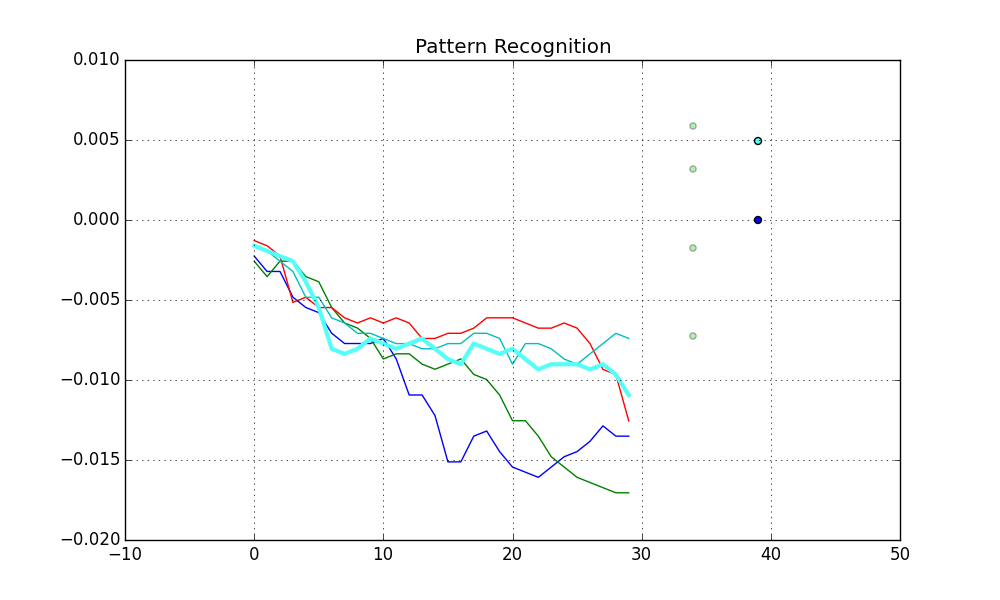
\includegraphics[scale=0.3]{figure_2}
        \caption{Examples of downward trend reversals}
\end{center}
\end{figure}

\begin{figure}[h!]
\begin{center}
        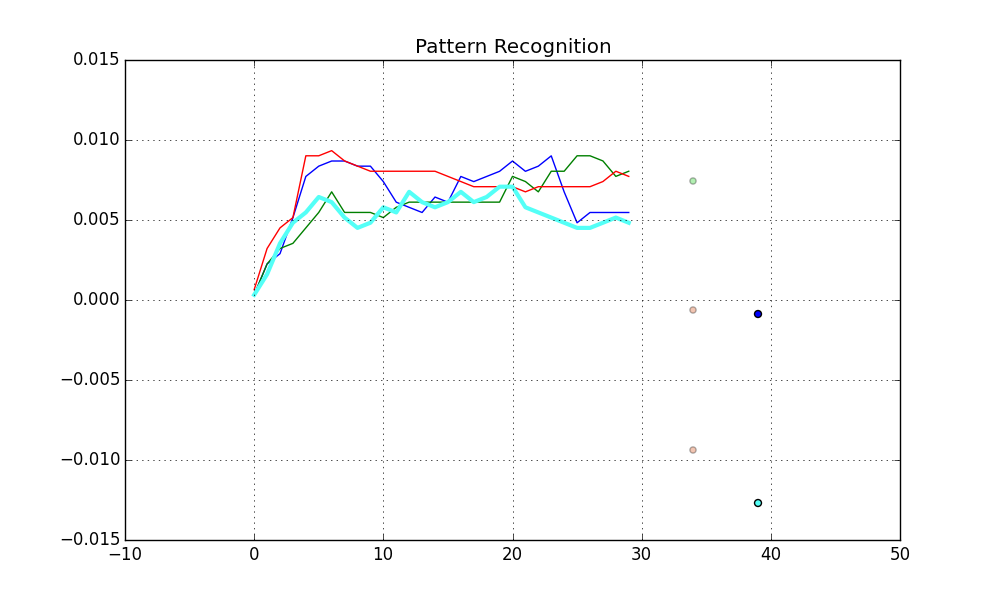
\includegraphics[scale=0.3]{figure_3}
        \caption{Examples of upward trend reversal}
\end{center}
\end{figure}

%You may want to include figures in the paper to help readers visualize
%your approach and your results. Such artwork should be centered,
%legible, and separated from the text. Lines should be dark and at
%least 0.5~points thick for purposes of reproduction, and text should
%not appear on a gray background.
%
%Label all distinct components of each figure. If the figure takes the
%form of a graph, then give a name for each axis and include a legend
%that briefly describes each curve. Do not include a title inside the
%figure; instead, be sure to include a caption describing your figure.
%
%You may float figures to the top or
%bottom of a column, and you may set wide figures across both columns
%(use the environment {\tt figure*} in \LaTeX), but always place
%two-column figures at the top or bottom of the page.
%
%\subsection{Algorithms}
%
%If you are using \LaTeX, please use the ``algorithm'' and ``algorithmic''
%environments to format pseudocode. These require
%the corresponding stylefiles, algorithm.sty and
%algorithmic.sty, which are supplied with this package.
%Algorithm~\ref{alg:example} shows an example.
%
%\begin{algorithm}[tb]
%   \caption{Bubble Sort}
%   \label{alg:example}
%\begin{algorithmic}
%   \STATE {\bfseries Input:} data $x_i$, size $m$
%   \REPEAT
%   \STATE Initialize $noChange = true$.
%   \FOR{$i=1$ {\bfseries to} $m-1$}
%   \IF{$x_i > x_{i+1}$}
%   \STATE Swap $x_i$ and $x_{i+1}$
%   \STATE $noChange = false$
%   \ENDIF
%   \ENDFOR
%   \UNTIL{$noChange$ is $true$}
%\end{algorithmic}
%\end{algorithm}
%
%\subsection{Tables}
%
%You may also want to include tables that summarize material. Like
%figures, these should be centered, legible, and numbered consecutively.
%However, place the title {\it above\/} the table, as in
%Table~\ref{sample-table}.
% Note use of \abovespace and \belowspace to get reasonable spacing
% above and below tabular lines.
%
%\begin{table}[h]
%\caption{Classification accuracies for naive Bayes and flexible
%Bayes on various data sets.}
%\label{sample-table}
%\vskip 0.15in
%\begin{center}
%\begin{small}
%\begin{sc}
%\begin{tabular}{lcccr}
%\hline
%\abovespace\belowspace
%Data set & Naive & Flexible & Better? \\
%\hline
%\abovespace
%Breast    & 95.9$\pm$ 0.2& 96.7$\pm$ 0.2& $\surd$ \\
%Cleveland & 83.3$\pm$ 0.6& 80.0$\pm$ 0.6& $\times$\\
%Glass2    & 61.9$\pm$ 1.4& 83.8$\pm$ 0.7& $\surd$ \\
%Credit    & 74.8$\pm$ 0.5& 78.3$\pm$ 0.6&         \\
%Horse     & 73.3$\pm$ 0.9& 69.7$\pm$ 1.0& $\times$\\
%Meta      & 67.1$\pm$ 0.6& 76.5$\pm$ 0.5& $\surd$ \\
%Pima      & 75.1$\pm$ 0.6& 73.9$\pm$ 0.5&         \\
%\belowspace
%Vehicle   & 44.9$\pm$ 0.6& 61.5$\pm$ 0.4& $\surd$ \\
%\hline
%\end{tabular}
%\end{sc}
%\end{small}
%\end{center}
%\vskip -0.1in
%\end{table}
%
%Tables contain textual material that can be typeset, as contrasted
%with figures, which contain graphical material that must be drawn.
%Specify the contents of each row and column in the table's topmost
%row. Again, you may float tables to a column's top or bottom, and set
%wide tables across both columns, but place two-column tables at the
%top or bottom of the page.

%Please use APA reference format regardless of your formatter
%or word processor. If you rely on the \LaTeX\/ bibliographic
%facility, use {\tt natbib.sty} and {\tt icml2014.bst}
%included in the style-file package to obtain this format.
%
%Citations within the text should include the authors' last names and
%year. If the authors' names are included in the sentence, place only
%the year in parentheses, for example when referencing Arthur Samuel's
%pioneering work \yrcite{Samuel59}. Otherwise place the entire
%reference in parentheses with the authors and year separated by a
%comma \cite{Samuel59}. List multiple references separated by
%semicolons \cite{kearns89,Samuel59,mitchell80}. Use the `et~al.'
%construct only for citations with three or more authors or after
%listing all authors to a publication in an earlier reference \cite{MachineLearningI}.
%
%The references at the end of this document give examples for journal
%articles \cite{Samuel59}, conference publications \cite{langley00}, book chapters \cite{Newell81}, books \cite{DudaHart2nd}, edited volumes \cite{MachineLearningI},
%technical reports \cite{mitchell80}, and dissertations \cite{kearns89}.
%
%Alphabetize references by the surnames of the first authors, with
%single author entries preceding multiple author entries. Order
%references for the same authors by year of publication, with the
%earliest first. Make sure that each reference includes all relevant
%information (e.g., page numbers).


\section*{Acknowledgments}

We would like to thank Eric Eaton and the TA's for their help with gathering data and getting started.

%f you did this work in collaboration with someone else, or if someone else (such as another
%professor) had advised you on this work, your report must fully acknowledge their contributions. If you received external help or assistance on this project, you must cite these sources here in the acknowledgements section.  If you do not have anything to list in this section, write simply ``None.''

\bibliography{example_paper}
\bibliographystyle{icml2014}

\end{document}


% This document was modified from the file originally made available by
% Pat Langley and Andrea Danyluk for ICML-2K. This version was
% created by Lise Getoor and Tobias Scheffer, it was slightly modified
% from the 2010 version by Thorsten Joachims & Johannes Fuernkranz,
% slightly modified from the 2009 version by Kiri Wagstaff and
% Sam Roweis's 2008 version, which is slightly modified from
% Prasad Tadepalli's 2007 version which is a lightly
% changed version of the previous year's version by Andrew Moore,
% which was in turn edited from those of Kristian Kersting and
% Codrina Lauth. Alex Smola contributed to the algorithmic style files.
